\documentclass[unicode,11pt,a4paper,oneside,numbers=endperiod,openany]{scrartcl}
\usepackage{amsmath}
\usepackage{listings}


\renewcommand{\thesubsection}{\arabic{subsection}}

\usepackage{ifthen}
\usepackage[utf8]{inputenc}
\usepackage{graphics}
\usepackage{graphicx}
\usepackage{hyperref}

\pagestyle{plain}
\voffset -5mm
\oddsidemargin  0mm
\evensidemargin -11mm
\marginparwidth 2cm
\marginparsep 0pt
\topmargin 0mm
\headheight 0pt
\headsep 0pt
\topskip 0pt        
\textheight 255mm
\textwidth 165mm

\newcommand{\duedate} {}
\newcommand{\setduedate}[1]{%
\renewcommand\duedate {\textbf{Due date:}~ #1}}
\newcommand\isassignment {false}
\newcommand{\setassignment}{\renewcommand\isassignment {true}}
\newcommand{\ifassignment}[1]{\ifthenelse{\boolean{\isassignment}}{#1}{}}
\newcommand{\ifnotassignment}[1]{\ifthenelse{\boolean{\isassignment}}{}{#1}}

\newcommand{\assignmentpolicy}{
\begin{table}[h]
\begin{center}
\scalebox{0.8} {%
\begin{tabular}{|p{0.02cm}p{16cm}|}
\hline
&\\
\multicolumn{2}{|c|}{\Large\textbf{Numerical Computing 2023 ---  Submission Instructions}}\\
\multicolumn{2}{|c|}{\large\textbf{(Please, notice that following instructions are mandatory: }}\\
\multicolumn{2}{|c|}{\large\textbf{submissions that don't comply with, won't be considered)}}\\
&\\
\textbullet & Assignments must be submitted to \href{https://www.icorsi.ch/course/view.php?id=14666}{iCorsi} (i.e. in electronic format).\\
\textbullet & Provide both executable package and sources (e.g. C/C++ files, MATLAB). 
If you are using libraries, please add them in the file. Sources must be organized in directories called:\\
\multicolumn{2}{|c|}{\textit{Project\_number\_lastname\_firstname}}\\
& and  the  file must be called:\\
\multicolumn{2}{|c|}{\textit{project\_number\_lastname\_firstname.zip}}\\
\multicolumn{2}{|c|}{\textit{project\_number\_lastname\_firstname.pdf}}\\
\textbullet &  The TAs will grade your project by reviewing your project write-up, and looking at the implementation you attempted, and benchmarking your code's performance.\\

\textbullet & You are allowed to discuss all questions with anyone you like; however: (i) your submission must list anyone you discussed problems with and (ii) you must write up your submission independently.\\
\hline
\end{tabular}
}
\end{center}
\end{table}
}
\newcommand{\punkte}[1]{\hspace{1ex}\emph{\mdseries\hfill(#1~\ifcase#1{Points}\or{Points}\else{Points}\fi)}}


\newcommand\serieheader[6]{
\thispagestyle{empty}%
\begin{flushleft}

\includegraphics[width=0.45\textwidth]{CI_logo}
\end{flushleft}
  \noindent%
  {\large\ignorespaces{\textbf{#1}}\hspace{\fill}\ignorespaces{ \textbf{#2}}}\\ \\%
  {\large\ignorespaces #3 \hspace{\fill}\ignorespaces #4}\\
  \noindent%
  \bigskip
  \hrule\par\bigskip\noindent%
  \bigskip {\ignorespaces {\Large{\textbf{#5}}}
  \hspace{\fill}\ignorespaces \large \ifthenelse{\boolean{\isassignment}}{\duedate}{#6}}
  \hrule\par\bigskip\noindent%  \linebreak
 }

\makeatletter
\def\enumerateMod{\ifnum \@enumdepth >3 \@toodeep\else
      \advance\@enumdepth \@ne
      \edef\@enumctr{enum\romannumeral\the\@enumdepth}\list
      {\csname label\@enumctr\endcsname}{\usecounter
        {\@enumctr}%%%? the following differs from "enumerate"
	\topsep0pt%
	\partopsep0pt%
	\itemsep0pt%
	\def\makelabel##1{\hss\llap{##1}}}\fi}
\let\endenumerateMod =\endlist
\makeatother




\usepackage{textcomp}





\begin{document}


\setassignment
\setduedate{Wednesday, 11 October 2023, 23:59 AM}

\serieheader{Numerical Computing}{2023}{\textbf{Student:} Hun Rim}{\textbf{Discussed with:} Georgy Batyrev}{Solution for Project 1}{}
\newline

\assignmentpolicy


\newpage

\subsection{Theoretical questions [15 points]}

\begin{enumerate}
\item[(a)] \textbf{What are an eigenvector, an eigenvalue and an eigenbasis?}\\
{Eigenvector : Eigenvector(i.e. \textit{v}) of a square matrix(i.e. \textit{A}) is a nonzero vector which linearly transforms in scale while staying in the same span when applied to the square matrix.}\\
\\
{Eigenvalue: Often expressed with $\lambda$, eigenvalue is a scalar which represents how much the eigenvector gets stretched when multiplied by a square matrix(\textit{A}). Although the direction doesn't change, the direction of the vector can be inverted from the transformation, hence, eigenvalue can be negative.}\\
To conclude, for a square matrix \textit{A} when applied to its eigenvector \textit{v}, the linear transformation can be represented as combination of the eigenvalue and the eigenvector.
\begin{center}
\begin{equation}
 Av = \lambda v
\end{equation}
\end{center}

{Eigenbasis: An eigenbasis of a square matrix(\textit{A}) is a \textbf{set of linearly independent eigenvectors} that spans the entire vector space of \textit{A}. Basically it is set of eigenvectors found from all eigenvalues corresponding to the square matrix.}
\item[(b)] \textbf{What assumptions should be made to guarantee convergence of the power method?}
For power method to guarantee a convergence, we need to assume that our power method is converging towards our dominant eigenvalue. Also we need to assume that the randomly chosen $x_0$, the initial vector, is is in the same direction as our eigenvector.
\item[(c)] \textbf{What is the shift and invert approach?}\\
{When $\lambda_2$, $\lambda_1$ are close, because the convergence is relative to asymptotic error constant $\mid \frac{\lambda_2}{\lambda_1} \mid$, the convergence can be very slow when it approaches 1. Hence, we use shift and invert (Inverse Iteration) approach to fasten the convergence for smaller problems as it has higher complexity (O($n^{3}$)) for computation but faster approach to convergence in comparison to power iteration(O($n^{2}$)).}\\

{For example, $\lambda_i$ are eigenvalue of \textit{A}, and $\lambda_i - \alpha$ are eigenvalue for \textit{A} - $\alpha$\textit{I}. Then, eigenvalue for $\textit{B} = (\textit{A} - \alpha\textit{I})^{-1}$ is $\mu_i = \frac{1}{\lambda_i - \alpha}$, while the eigenvectors remain unchanged.
If we apply power method to \textit{B}, the new convergence rate will be $\mid \frac{\mu_2}{\mu_1} \mid$ = $\mid \frac{\lambda_1 - \alpha}{\lambda_2 - \alpha} \mid$. Hence, choosing $\alpha \approx \lambda_1$ is very beneficial and common as it brings rapid convergence. }
\item[(d)] \textbf{What is the difference in cost of a single iteration of the power method, compared to the inverse iteration?}\\
{When solving a power method, we need to carry out matrix-vector multiplication, which has a time complexity of $O(n)^{2}$ like I mentioned in the previous answer. When solving an inverse iteration, we need to solve a linear system which has a time complexity of $O(n)^{3}$. Obviously, inverse iteration has far more severe time complexity in comparison to power method even though it has more rapid convergence. Hence, inverse method is recommended for smaller problems.}
\item[(e)] \textbf{What is a Rayleigh quotient and how can it be used for eigenvalue computations?}\\
{The Rayleigh quotient is a possible improvement on inverse iteration method when computing the eigenvalues. It guarantees upto cubic function when approaching the convergence. They achieve this quick approaching speed via replacing $\alpha$ with Rayleigh quotient in each iteration. As Rayleigh quotient has to refactor the matrix every iteration, it has higher time complexity but the benefits are worthwhile.}
\begin{center}
\begin{equation}
 R(v) = \frac{v^{T}Av}{v^{T}v}
\end{equation}
\end{center}

\end{enumerate}

\subsection{Connectivity matrix and subcliques [5 points]}
\begin{center}
 \begin{tabular}{|c | c|}
 \hline
 Range & Dominant Links \\ \hline
 73 - 100 & http://www.baug.ethz.ch \\ \hline
 113 - 130 & http://www.math.ethz.ch \\ \hline
 164 - 182 & http://www.mavt.ethz.ch \\ \hline
 198 - 220 & http://www.biol.ethz.ch \\ \hline
 221-263 & http://www.chab.ethz.ch \\ \hline
 264 - 315 & http://www.math.ethz.ch \\ \hline
 319 - 348 & http://www.erdw.ethz.ch \\ \hline
 350 - 356 & http://www.hest.ethz.ch \\ \hline
 359 - 373 & http://www.usys.ethz.ch \\ \hline
 385 - 393 & http://www.usys.ethz.ch \\ \hline
 396 - 416 & http://www.mtec.ethz.ch \\ \hline
 426 - 431 & http://www.mtec.ethz.ch \\ \hline
 436 - 461 & http://www.gess.ethz.ch \\ \hline
 488 - 500 & http://www.bilanz.ch \\ \hline
 \end{tabular}

\end{center}
\subsection{Connectivity matrix and disjoint subgraphs [10 points]}

\begin{center}
  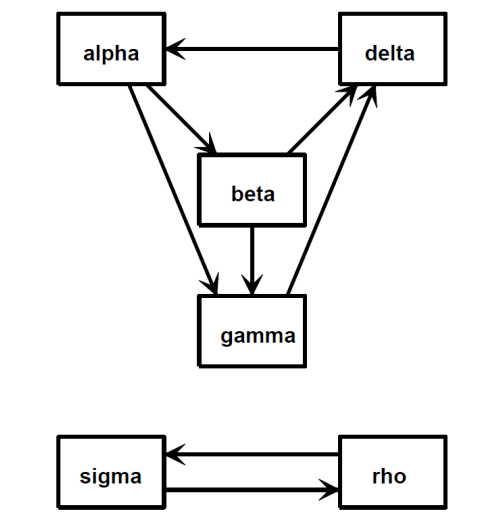
\includegraphics[width=0.5\linewidth]{./images/figure7.png}\\
  \label{fig:Another tiny Web}
  {Figure 1: The tiny web}
\end{center}

\begin{enumerate}
 \item {What is the connectivity matrix G? Which are its entries?} \\
 
 Following the example given in the Project description page:\\
 
 {U = ['alpha', 'beta', 'gamma', 'delta', 'rho', 'sigma']}\\
 {i = [2, 3, 3, 4, 4, 1, 6, 5]}\\
 {j = [1, 1, 2, 2, 3, 4, 5, 6]}\\
 {n = 6 \\ G = sparse(i, j, 1, n, n)}\\
 
 {To briefly describe the variables, \textit{U} is the array of shortened URLs, \textit{i} is the array of destination URLs in-terms of its index in the URL array, and \textit{j} is the array of starting point URLs in same context as the destination URLs. Naturally, \textit{n} is the dimension of connectivity matrix (\textit{G}) as the tiny web consists of 6 websites. Finally, the connectivity matrix is formed using a sparse matrix depicting the relation between 2 vectors \textit{i, and j} in a $n \times n$ matrix format. When we call the \textit{full(G)} to see the $n \times n$ format of connectivity matrix \textit{G}, we get the following result: (Assuming we follow the row and column order according to the elements of the vector \textit{U})}
 
\begin{center}
{ \textit{G =}
$\begin{pmatrix}
 0 & 0 & 0 & 1 & 0 & 0 \\
 1 & 0 & 0 & 0 & 0 & 0 \\
 1 & 1 & 0 & 0 & 0 & 0 \\
 0 & 1 & 1 & 0 & 0 & 0 \\
 0 & 0 & 0 & 0 & 0 & 1 \\
 0 & 0 & 0 & 0 & 1 & 0 \\
\end{pmatrix}$
}
\end{center}

\item {What are the PageRanks if the hyperlink transition probability p assumes the default value of 0.85?} \\

{Knowing our transition probability \textit{p = 0.85}, we can use the given function,\textbf{ pagerank}, from \textit{pagerank.m} MATLAB script and call the following on MATLAB command window to get the PageRanks of our imaginary \textbf{tiny web}:}

 $f_x >>$ \textit{p = 0.85} \\
 $f_x >>$ \textit{pagerank(U, G, p)} \\
 
 {Using arrays \textit{U, G,} which are reutilized, the result will be the following: }
 
 \begin{center}
  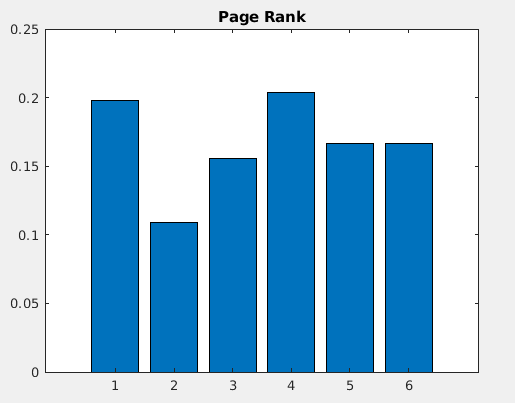
\includegraphics[width=0.5\linewidth]{./images/4_2.png}\\
  \label{fig:PageRank of nodes in the tiny web}
  {Figure 2: Barchart for pagerank of nodes in the tiny web (figure 1)}
 \end{center}

 {If we summarize the bar graph data, and connectivity matrix data into a table, we get the following: }\\
 
 \begin{center}
  

 \begin{tabular}{| c | c | c | c | c |}
 \hline
 Index & U & PageRank & Incoming & Outgoing \\
 \hline
 1 & alpha & 0.19814 & 1 & 2 \\
 \hline
 2 & beta & 0.109209 & 1 & 2 \\
 \hline
 3 & delta & 0.155623 & 2 & 1 \\
 \hline
 4 & gamma & 0.203694 & 2 & 1 \\
 \hline
 5 & rho & 0.166667 & 1 & 1 \\
 \hline
 6 & sigma & 0.166667 & 1 & 1 \\
 \hline
 \end{tabular}
 \\
 \vspace{5px}
 {Figure 3: Summarized table for pagerank of nodes in the tiny web}
 \end{center}
 
 \item {Describe what happens with this example to both the definition of PageRank and the computation done by
pagerank in the limit p → 1.}\\

 \begin{center}
  

 \begin{tabular}{| c | c | c | c | c | c | c |}
 \hline
 Index & U & PR(0.85) & PR(0.00) & PR(0.999999) & In & Out\\
 \hline
 1 & alpha & 0.19814 & 0.166667 & 0.205128 & 1 & 2 \\
 \hline
 2 & beta & 0.109209 & 0.166667 & 0.102564 & 1 & 2 \\
 \hline
 3 & delta & 0.155623 & 0.166667 & 0.153846 & 2 & 1 \\
 \hline
 4 & gamma & 0.203694 & 0.166667 & 0.205128 & 2 & 1 \\
 \hline
 5 & rho & 0.166667 & 0.166667 & 0.166667 & 1 & 1 \\
 \hline
 6 & sigma & 0.166667 & 0.166667 & 0.166667 & 1 & 1 \\
 \hline
 \end{tabular}
 \\
 \vspace{5px}
 {Figure 4: Summarized table for pagerank(s) of nodes in the tiny web (PR: PageRank)}
 \end{center}
 
 {\textit{p} is the probability that the random walk follows a link(edge) and (1 - \textit{p}) is the probability that it leads to an arbitrary page. \\
 Hence, if \textit{p → 0} all the pages have the same pagerank as it always leads to an arbitrary page, and all the pages have the same pagerank as it always leads to a random website in the web. When \textit{p → 1}, because the possibility of leading to an arbitrary page is negligible, pagerank directly correlates to incoming link's pagerank and their number of outgoing links. I.e. alpha has two outgoing hyperlinks so beta's pagerank is exactly half of alpha unlike when \textit{p → 0.85}. Furthermore, usually delta and alpha's pagerank are very close but never same as there are constant factors added to their pagerank due to the possibility of going to a random page. \\ However, When \textit{p} converges to 1, because there are negligible chance of being directed to an arbitrary page, it simplifies the computation of pageranks. \\
 
 Problem with \textit{p} being 0, is that in this sort of web (disjoint graph), it would become impossible to traverse some parts of the graph.}

\end{enumerate}

\subsection{PageRanks by solving a sparse linear system [25 points]}
\begin{enumerate}
 \item Create \textit{pagerank1.m} by modifying \textit{pagerank.m} to use \textbf{the power method} instead of solving the sparse linear system. The key statements are : \\
 \begin{lstlisting}[language=Matlab]
 G = p * G * D;
 z = ((1-p) * (c~=0) + (c==0)) / n;
 while termination_test
    x = G * x + e * (z * x);
 end
 \end{lstlisting}
 What is an appropriate test for terminating the power iteration?\\
 
 In the default section, I implemented the following code:
 \begin{lstlisting}[language=Matlab]
    z = ((1-p) * (c~=0) + (c==0)) / n;
    A = p * G * D + e * z; 
    x = e / n;
    oldx = zeros(n, 1);
    limit = 0.00001;
    while norm(x - oldx) > limit
        oldx = x;
        x = A * x;
    end
    x = x / sum(x);
  
 \end{lstlisting}
 
 As it can be seen from the code implementation, the while loop continues the iteration while:
 \begin{lstlisting}[language=Matlab]
  norm(x - oldx) > limit
 \end{lstlisting}
 
 Meaning, the iteration gets terminated when the normal between old and new \textit{x} converges to the given limit and goes below it. (which in this case was 0.01)
 
 \item Create \textit{pagerank2.m} by modifying \textit{pagerank.m} to use the inverse iteration. The key statements are:
 \begin{lstlisting}[language=Matlab]
  while termination_test
    x = (alpha * I - A) \ x;
    x = x / sum(x, 1);
  end
 \end{lstlisting}
 
 Use your functions pagerank1.m and pagerank2.m (set $\alpha$ = 0.99) to compute the PageRanks of the six-node example presented in Figure 1. Make sure you get the same result from each of your three functions.\\
 
 \begin{center}
  

  \begin{tabular}{| c | c | c | c | c | c | c | c |}
 \hline
 Index & U & PR(figure 1) & PR & PR1 & PR2 & In & Out\\
 \hline
 1 & alpha & 0.3210 & 0.3210 & 0.3210 & 0.3210 & 2 & 2 \\
 \hline
 2 & beta & 0.1705 & 0.1705 & 0.1705 & 0.1705 & 1 & 2 \\
 \hline
 3 & delta & 0.1066 & 0.1066 & 0.1066 & 0.1066 & 1 & 3 \\
 \hline
 4 & gamma & 0.1368 & 0.1368 & 0.1368 & 0.1368 & 2 & 1 \\
 \hline
 5 & rho & 0.0643 & 0.0643 & 0.0643 & 0.0643 & 1 & 0 \\
 \hline
 6 & sigma & 0.2007 & 0.2007 & 0.2007 & 0.2007 & 2 & 1 \\
 \hline
 \end{tabular}\\
 \vspace{5px}
 {Figure 5: Result of computing PR for figure 1 (in project file) data using all 3 pageranking scripts.}
 \end{center}

 {implementation for \textit{pagerank2.m}, Inverse iteration method is as following: }\\
 
 \begin{lstlisting}[language=Matlab]
    z = ((1-p)*(c~=0) + (c==0))/n;
    disp('Using Inverse Iteration Implementation')
    x = e / n;
    A = p * G * D + (e * z);
    oldx = zeros(n, 1);
    limit = 0.00001;
    alpha = 0.99;
    while norm(x - oldx) >= limit
        oldx = x;
        x = (alpha * I - A) \ x;
        x = x/sum(x);
    end
 \end{lstlisting}
 
 \item {We now want to analyse the impact of $\alpha$ on the inverse iteration. Using the ETH500 example, set $\alpha$ equal
to 0.8, 0.9, 0.95 and 1. Comment on the different number of iterations the four cases take until convergence.
Analyse your results and explain what you observe.}\\

\begin{center}
 \begin{tabular}{| c | c | c | c | c | c |}
 \hline
 & $\alpha$ = 0.99 & $\alpha$ = 0.95 & $\alpha$ = 0.92 & $\alpha$ = 0.915 & $\alpha$ = 0.9, 0.8 \\
 \hline
 Iteration Count & 5 & 11 & 28 & 38 & NaN generated\\
 \hline
 \end{tabular}
 \\ \vspace{5px}
{Figure 6: Iteration count for different values of $\alpha$ when limit is $10^{-5}$}
\end{center}

{From limited data observed through inverse iteration algorithm ($\alpha = 0.92, 0.915$ are added for better analysis), we can observe that the $\alpha$ is inversely proportional to iteration count, because as $\alpha$ decreases, iteration count till convergence increases as it is moving away from $\lambda$. Also the iteration count exponentially increases as $\alpha$ gets smaller. Furthermore, after certain value of $\alpha$ (between 0.9 to 0.915), it becomes incomputable.}

\item {Use your functions \textit{pagerank1.m} and \textit{pagerank2.m} (set $\alpha$ = 0.99) to compute the PageRanks of three
selected graphs \textit{(web1.mat, web2.mat and web3.mat)}. Report on the convergence of the two methods
for these subgraphs and summarize the advantages and disadvantages of the power method implemented in
\textit{pagerank1.m against the inverse iteration in pagerank2.m}.} \\

After running power method algorithm and inverse iteration algorithm on 3 different data sets (\textit{web1.mat, web2.mat, web3.mat}) it became clear inverse iteration goes through immensely less number of iterations to reach the converging point. However, to measure the two algorithm's performance more accurately, their average execution time is also measured.

\begin{center}
 \begin{tabular}{| c | c | c | c | c |}
 \hline
 Dataset & PR1 Iteration & PR1 Run Time(avg) & PR2 Iteration & PR2 Run Time(avg) \\
 \hline
 \textit{web1.mat} & 145 & 0.0518 & 14 & 0.0682 \\
 \hline
 \textit{web2.mat} & 145 & 0.0532 & 14 & 0.0668 \\
 \hline
 \textit{web3.mat} & 212 & 0.0432 & 15 & 0.0675 \\
 \hline
 \end{tabular}\\
 \vspace{5px}
{Figure 7: Table showing iteration count and average execution time of reaching convergence using power method and inverse iteration}
\end{center}

{The average execution time was measured using $timeit(func())$ function built into the MATLAB, which takes a pointer to a function and outputs the function's average execution time after running it numerous times.}\\

{To clearly see the execution time difference, the convergence limit was set to $10^{-17}$ and as it can be seen from the table above, even though power method clearly exceeds inverse iteration in terms of iteration count (lower is better), the average execution time of inverse iteration method is $30^{+}\%$ higher (lower is better) than power method. To conclude, power method provides faster results as advantages although it requires more iterations.}
\end{enumerate}


\subsection{The Reverse Cuthill--McKee Ordering [5 points]}

{\textbf{Visualization of Matrices:}\\
The sparsity pattern of the original and permutted $A\_SymPosDef$ matrices are shown below:} \\

 \begin{center}
  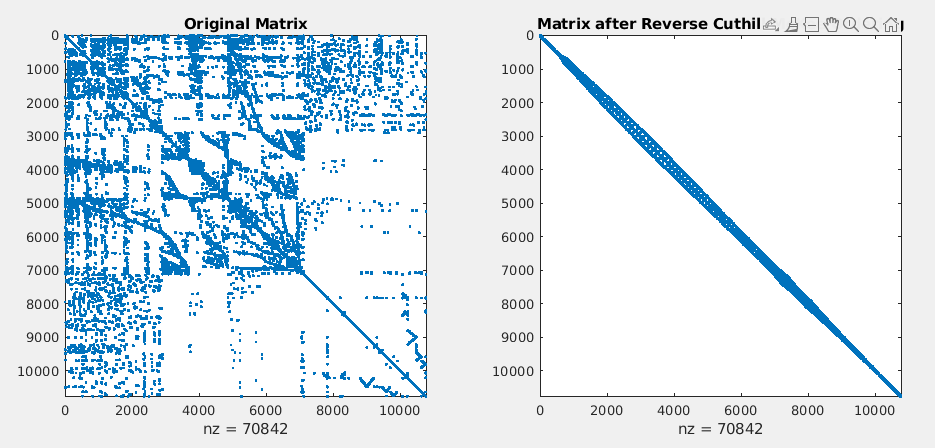
\includegraphics[width=0.5\linewidth]{./images/q5original.png}\\
  \label{fig:PageRank of nodes in the tiny web}
  {Figure 8: Spy graphs of original matrix (left) and matrix after Reverse Cuthill McKee permutation(right)}
 \end{center}
 
 {From the figure above we can observe the way sparse values, covering large area have been minimized to a denser, smaller area.}\\
 \newpage
 
 {\textbf{Visualization of Cholesky Factors}}
 
  \begin{center}
  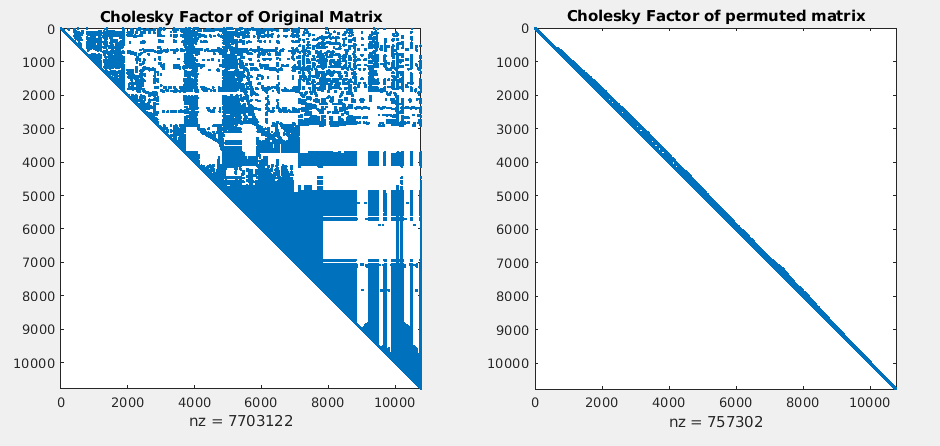
\includegraphics[width=0.5\linewidth]{./images/q5cholesky.png}\\
  \label{fig:PageRank of nodes in the tiny web}
  {Figure 9: Original Matrix after Cholesky decomposition,(left) and Permutted matrix after Cholesky decomposition(right)}\\
 \end{center}
 
  {From figure 9, we may observe the similar pattern of behavior as in graph above. Interestingly, it is important to note that if the matrix must be positive definite using eigenvalues, else we can't compute Cholesky Factorization. (To recreate the graphs, please run \textit{reverse.m} script)}


\subsection{Sparse Matrix Factorization [10 points]}
{Let $A \in R^{n\times n}$ be symmetric and positive definite, with entries $A_ij$ defined as follows:}\\
\begin{equation}
A_{ij}=
\begin{cases}
    1 \hspace{55px} if \hspace{11px}i = 1 \hspace{11px} or \hspace{11px} i=n \hspace{11px} or \hspace{11px} j=1 \hspace{11px} or \hspace{11px} j=n \hspace{11px} and \hspace{11px} i\neq j \\
    n + i - 1 \hspace{17px} if \hspace{11px} i=j\\
    0 \hspace{55px} otherwise
\end{cases}
\end{equation}

{Please note that the increasingly larger values on the diagonal are necessary to ensure the positive definiteness of
matrix A.}\\

\begin{enumerate}
 \item {Construct matrix A for the case n = 10 and explicitly write down its entries. How many non-zero elements does it have?} \\
 {According to the given $A_{ij}$ equation, when n = 10, the matrix A is as following:}
 \begin{center}
{ \textit{A =}
$\begin{pmatrix}
 10 & 1 & 1 & 1 & 1 & 1 & 1 & 1 & 1 & 1 \\
 1 & 11 & 0 & 0 & 0 & 0 & 0 & 0 & 0 & 1 \\
 1 & 0 & 12 & 0 & 0 & 0 & 0 & 0 & 0 & 1 \\
 1 & 0 & 0 & 13 & 0 & 0 & 0 & 0 & 0 & 1\\
 1 & 0 & 0 & 0 & 14 & 0 & 0 & 0 & 0 & 1 \\
 1 & 0 & 0 & 0 & 0 & 15 & 0 & 0 & 0 & 1 \\
 1 & 0 & 0 & 0 & 0 & 0 & 16 & 0 & 0 & 1 \\
 1 & 0 & 0 & 0 & 0 & 0 & 0 & 17 & 0 & 1 \\
 1 & 0 & 0 & 0 & 0 & 0 & 0 & 0 & 18 & 1 \\
 1 & 1 & 1 & 1 & 1 & 1 & 1 & 1 & 1 & 19 \\
\end{pmatrix}$
}
\end{center}
{The square matrix A has 56 entries which are zero and 44 entries which are non-zero values. }\\

\item {We now want to derive a general formula to compute the number of non-zero entries. Show that, for a given matrix $A \in R^{n \times n}$ with this structure, the number of non-zero elements are $5n - 6$.}

{Fundamently, number of non-zero elements equal to: \\

\textit{elements on the border of matrix + element on left-to-right diagonal - overlapping elements} \\

Their are n elements on each borders and the diagonal so:}\\
\begin{center}
\begin{equation}
 total-non-zero-entries = 4n + n - \alpha = 5n - \alpha
\end{equation}
\end{center}

{Where $\alpha$ equals to number of overlapping elements.}\\
{If we count all the borders of a square matrix, each of the edges will be counted twice so we need to minus four from our $5n$, now when we count the non-zero entries on the diagonal on top of our calculation made on entries on the border, two edges where $i=j, i=1,n$ will overlap once each. Hence, we need to minus another two from our $5n - 4$. Finally we get:}
\begin{center}
\begin{equation}
 total-non-zero-entries = 5n - 4 - 2 = 5n - 6
\end{equation}
\end{center}

\item Write a function \textit{A\_construct()}, which takes as input n and returns, as output, the matrix A defined in Eq. 3 and its number of non-zero elements nz. Test your function in a script \textit{ex2c.m for n = 10} and compare
your results with those you obtained in point (a). Furthermore, within the same script, visualise the non-zero
structure of matrix A by using the command \textit{spy()}.\\

\begin{center}
  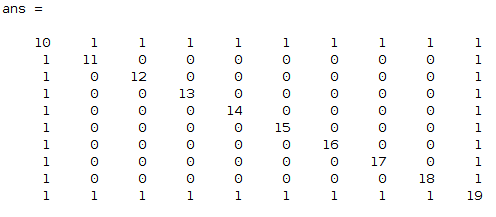
\includegraphics[width=0.5\linewidth]{./images/n10matrix.png}\\
  \label{fig:Resultant matrix}
  {Figure 10: Result matrix of \textit{A\_construct(n = 10)} function}
\end{center}

{As it can be seen, resultant matrix of the \textit{A\_construct(10)} has identical entries as the answer to question 6.1, and the following is the spy graph of the function: }

\begin{center}
  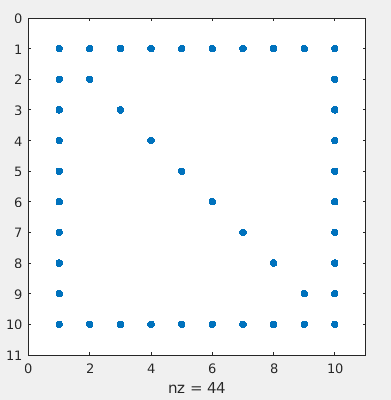
\includegraphics[width=0.5\linewidth]{./images/n10spy.png}\\
  \label{fig:Resultant spy graph}
  {Figure 11: Result spy graph of \textit{A\_construct(n = 10)} function}
\end{center}

{The function \textit{A\_construct()} has time complexity of $O(n^2)$. In the code below, to express inequality an exclamation mark($!=$) is used for readability, but in MATLAB tilde($\sim =$) symbol is used.}

\begin{lstlisting}[language=Matlab]
    function nnm = A_construct(n)
        A = sparse(zeros(n,n));
        for i = 1:n
            for j = 1:n
                if (i == 1 || i == n || j == 1 || j == n) && i != j
                    A(i, j) = 1;
                elseif i == j
                    A(i, j) = n + i - 1;
                end
            end
        end
        nnm = A;
    end
\end{lstlisting}

\item {Using again the \textit{spy()} command, visualize side by side the original matrix A and the result of the \textit{Cholesky factorization (chol() in Matlab)}.} \\
\begin{lstlisting}[language=Matlab]
    original = A_construct(10);
    cholesky = chol(original);
    tiledlayout(1, 2);
    nexttile
    spy(original);
    title('Original Matrix Spy Graph');
    nexttile
    spy(cholesky);
    title('Cholesky Factorization Spy Graph');
\end{lstlisting}

\begin{center}
  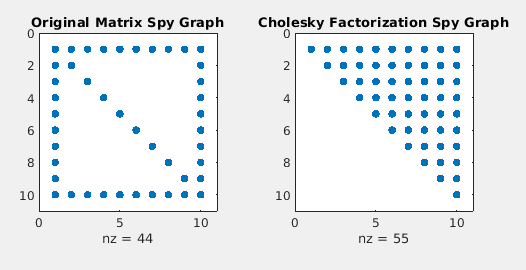
\includegraphics[width=0.8\linewidth]{./images/n10OC.png}\\
  \label{fig:Original and Cholesky factorization graphs}
  {Figure 12: Original Matrix Spy Graph[left], Result Of Cholesky Factorization [Right]}
\end{center}

{The graphs above is generated by a MATLAB script stored in \textit{original\_cholesky.m} file using the code given in the previous page.}

\item Explain why, for $n = 100, 000$, using \textit{chol()} to solve $Ax = b$ for a given right-hand-side vector \textit{b} would be problematic. Are there ways to mitigate this issue?

{There are serious problem behind solving Cholesky factorization using $Ax = b$ for a given right-hand-side vector \textit{b}.}
\begin{enumerate}
 \item With this method, you need to store both original matrix (let's call it \textit{A}) and the lower triangle (\textit{L}). Considering square matrix A has size $n \times n$ where $n = 100,000$ and it has to store \textit{L} of the same size, it may exceed the given memory limit.
 \item Also it has a very high time complexity. The computation has a cost of $O(n^{3})$. For a square matrix with row and column size of $n = 100,000$, it is a very costly and inefficient operation.
\end{enumerate}

{To mitigate the issue highlighted above, there are few solutions.}
\begin{enumerate}
 \item If we use sparse matrix and algorithm fit for it, for matrices containing a lot of zeros, it will significantly reduce both space and time complexity.
 \item Secondly, it is also possible to divide the problem into smaller pieces and use parallelization to solve the problem using multiple threads, fastening the computation speed.
 \item Thirdly, it is possible to take a more iterative approach more suited for larger sparse systems such as \textit{Conjugate Gradient(CG) Method}, instead of solving the system directly using Cholesky decomposition.
\end{enumerate}
\end{enumerate}


\subsection{Degree Centrality [5 points]}
\begin{lstlisting}[language=Matlab]
    load('householder/housegraph.mat');
    degree = sum(A, 2);
    [degreeSorted, indexNames] = sort(degree);
    count = length(degreeSorted);
    maxDegree = degreeSorted(count);
    coauthors = strings(5, maxDegree)
    authors = strings(5, 1);
    k = 1;
    for i = count : -1 : count - 4 
        ind = indexNames(i);
        j = 1;
        while ~isspace(name(ind, j))
            authors(k) = strcat(authors(k), name(ind, j));
            j = j + 1;
        end
        k = k + 1;
    end
    
    l = 1;
    for i = count: -1 : count -4
        nameCount = 1;
        ind = indexNames(i);
        for j = 1 : count
            if (A(ind, j) == 1)
                k = 1
                while ~isspace(name(j, k))
                    coauthors(l, nameCount) = strcat
                        (coauthors(l, nameCount), name(j, k));
                    k = k + 1;
                end
                nameCount = nameCount + 1;
            end
        end
    l = l + 1;
    end
    
\end{lstlisting}

{By executing the code above through \textit{degreeOfCentrality.m} script, it is possible to see the top 5 authors from the \textit{authors variable} and their coauthros from the \textit{coauthors variable}. The table below shows a summary of gathered information: }\\
\vspace{30px}
\begin{center}
\begin{tabular}{| c | c | c | c |}
\hline
 Degree Of Centrality & Index & Author & Co-authors \\
 \hline
 32 & 1 & Golub & Golub, Wilkinson, TChan, Varah, Overton etc. \\
 \hline
 16 & 104 & Demmel & Edelmen, VanLoan, Bai, Schreiber, Kahan etc. \\
 \hline
 14 & 86 & Plemmons & Golub, Nagy, Harrod, Pan, Funderlic etc. \\
 \hline
 13 & 81 & Heath & Golub, TChan, Funderlic, George, Gilbert etc. \\
 \hline
 13 & 44 & Schreiber & TChan, VanLoan, Moler, Gilber, Pothen etc. \\
 \hline
\end{tabular}\\
\vspace{5px}
{Figure 13: Table of authors and their coauthors sorted according to author's degree of centrality}.\\
\end{center}
\vspace{30px}

\subsection{The Connectivity of the Coauthors [5 points]}

{How many coauthors have the authors in common? Think about a general procedure that allows you to compute the list of common coauthors of two authors and express it in matrix notation. Use the formula you derived to compute the common coauthors of the pairs (Golub, Moler), (Golub, Saunders), and (TChan, Demmel). Who are these common coauthors? Report their names.}\\

{The solution is very straight forward. From the connectivity matrix \textit{A} which contains all the connection between authors and coauthors, if two author's columns have 1(have connection) on the same row, it means they have a common coauthor. From this logical process we can define the common coauthors between two authors as following:}\\
\begin{center}
\begin{equation}
commonCoauthorIndex = A(col: author_1) \cap A(col: author_2)
\end{equation}\\
\end{center}
\vspace{30px}

{If this logic is implemented as a script in MATLAB(view \textit{ex8.m} script for the code), we get the following results:}\\

\begin{center}
\begin{tabular}{| c | c | c |}
\hline
 Author1 & Author2 & Common Coauthors \\
 \hline
 Golub & Moler & Wilkinson, VanLoan \\
 \hline
 Golub & Saunders & Golub, Saunders, Gill \\
 \hline
 TChan & Demmel & Schreiber, Arioli, Duff, Heath\\
 \hline
\end{tabular}\\
\vspace{5px}
{Figure 14: Table of authors and their common co-authors}\\
\end{center}

\newpage

\subsection{PageRank of the Coauthor Graph [5 points]}

\begin{center}
  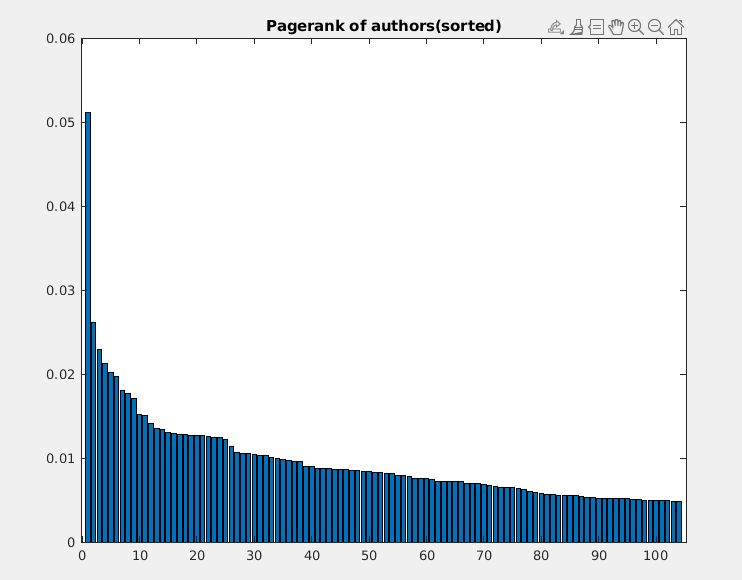
\includegraphics[width=0.5\linewidth]{./images/ex9.png}\\
  \label{fig:Pagerank of authors sorted(descending)}
  {Figure 15: Pagerank of authors sorted(descending)}
\end{center}

{The graph has been generated from the following script below using the given pagerank script as part of the project package.}
\vspace{10px}

\begin{lstlisting}[language=Matlab]
    load('householder/housegraph.mat');
    U = cellstr(name);
    authorRanks = pagerank(U, A, 0.85);
    sortAuthorRank = sort(authorRanks);
    sortAuthorRank = flip(sortAuthorRank);
    bar(sortAuthorRank);
    title('Pagerank of authors(sorted)');
        
\end{lstlisting}
\vspace{10px}

{The script simply uses A as the connectivity matrix and generates the pagerank as authorRanks variable. First it is sorted in ascending order and it is flipped using a flip() function and displayed as a bar graph.}\\

% \subsection{Quality of the Report [15 points]}
\vspace{100px}
{\textbf{All the MATLAB script used during this project are stored in the src folder.}}




\end{document}
